

%%%%
\section{Exploratory graphics}
\label{exploratoryGraphicsSection}

Many interesting analyses draw on multiple sources or creative representations of graphics. This sections three graphical explorations of the 2008-9 financial crisis, the relationship among and 2011-2012 GOP presidential nomination race, and three variables of the \data{states} data set: \var{smoking}, \var{murder}, and \var{coalEnergy} (the percent of a state's energy that comes from coal).

So far we have focused largely on one source of data at a time. Many of the most interesting analyses and insights are generated by merging data across sources.

\subsection{2008-9 financial crisis}

In this section, we combine Wikipedia data with financial data to consider the impact financial markets had on the public's interest in understanding what is a \emph{financial crisis}. Wikipedia's traffic is publicly available on \href{http://stats.grok.se/}{stats.grok.se}, and stock information can be downloaded from a website like \href{http://www.google.com/finance}{Google Finance} or \href{http://finance.yahoo.com/}{Yahoo! Finance}. We will take a look at why one might be interested in merging these data.

Figure~\ref{wikipediaStocks} shows visit's to  \href{http://en.wikipedia.org/wiki/Financial_crisis}{Wikipedia's Financial Crisis page} and the Dow Jones Industrial Average (DJI) from late 2007 until early 2012. The DJI is a stock index and is a good indicator of a large number of stocks. That is, if it goes down, that means many stocks also went down, and so on.
\begin{figure}
   \centering
   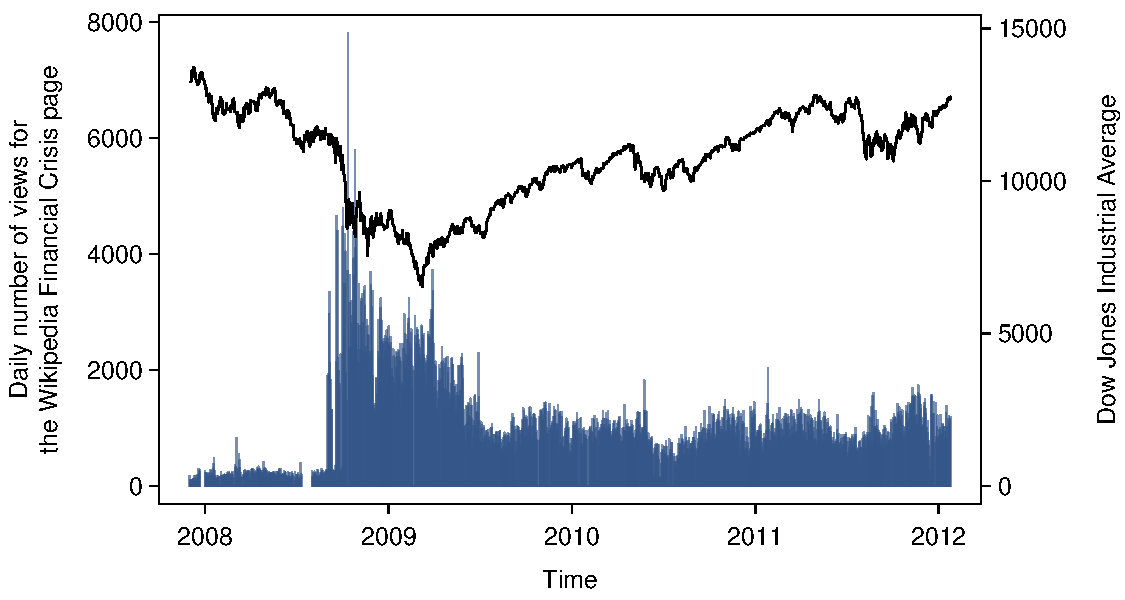
\includegraphics[width=\textwidth]{01/figures/wikipediaStocks/wikipediaStocks}
   \caption{The vertical lines show the number of daily views of Wikipedia's Financial Crisis page from late 2007 to early 2012, where the scale . Any regions with missing spikes indicate dates where data is missing. The continuous line that dips and rises represents the daily closing price of the Dow Jones Industrial Average, which represents.}
   \label{wikipediaStocks}
\end{figure}
% Peak	2007-10-09	14,164.53
% 		2008-09-01	11,543.55 (round to 11,500 since this was a weekend)
%		2008-10-01

Let's take the data separately before we analyze their joint information. In the DJI, a general decline in stocks is evident until a bottoming out in the first quarter of 2009. From there forward, there is a general increase in the index, albeit the increase is regularly interrupted by drops in price.

The page view data tells another interesting account of the financial crisis. There were few visitors to the financial crisis page until late 2008 when views soared. There was a peak in visitors before 2009, which declined to an elevated but much more stable number of views in mid-2009.

If the combined data is actually shocking. The financial crisis page views occurred immediately before the steepest sell-offs. The first day with more than 1000 page views was September 1st when the DJI was off by 19\% from its October 2007 peak (14,165). By October 15th, 2008, the DJI would drop a further 21\%, at which point page views were soaring to over 4000 each day, up from the August average of 203 page views each day. By the time the DJI index bottomed out, it lost over 53\% of its

The story told by these data is intriguing. Based on this example, it might be tempting to predict stock movements or other outcomes based on page view data. We want to temper this sentiment a little by noting that other page views may not always be so clear. For instance, a company's Wikipedia page may have a surge in views, which might indicate success, dramatic failure, or nothing of meaningful whatsoever. As we learned in Section~\ref{}, trying to identify causal relationships from observational data is at best, very difficult, and at worst, impossible.


%\subsection{GOP presidential nomination race}

\subsection{Debt ceiling deadline}

Summer 2011 saw one of the most heated and controversial political battles that roiled global financial markets and contributed to the first downgrade of United States debt. We can take a glimpse inside of the political back-and-forth by examining the Twitter profiles of three of the most prominent political players in the debate: President Barack Obama, Speaker John Boehner, and Senate Minority Leader Mitch McConnell. Figure~\ref{} shows their weekly number of Twitter posts.



